% Created 2021-12-06 Mon 01:53
% Intended LaTeX compiler: pdflatex
\documentclass[presentation, aspectratio=54]{beamer}
\usepackage[utf8]{inputenc}
\usepackage[T1]{fontenc}
\usepackage{graphicx}
\usepackage{grffile}
\usepackage{longtable}
\usepackage{wrapfig}
\usepackage{rotating}
\usepackage[normalem]{ulem}
\usepackage{amsmath}
\usepackage{textcomp}
\usepackage{amssymb}
\usepackage{capt-of}
\usepackage{hyperref}
\AtBeginSection[]{\begin{frame}\frametitle{}\LARGE\insertsectionhead\vspace{0.1cm}\hrule\end{frame}}
\usepackage{eso-pic}% http://ctan.org/pkg/eso-pic
\renewcommand{\Large}{\large}
\usetheme{Montpellier}
\usecolortheme{wolverine}
\usefonttheme[stillsansserifsmall,stillsansseriflarge,structure]{serif}
\author{Ing. Stalin Francis}
\date{\today}
\title{Fundamentos de programación}
\newcommand\AtPagemyUpperLeft[1]{\AtPageLowerLeft{\put(\LenToUnit{0.85\paperwidth},\LenToUnit{0.9\paperheight}){#1}}}\AddToShipoutPictureFG{\AtPagemyUpperLeft{{
\includegraphics[width=1.cm,keepaspectratio]{logo-utlvte.png}}}}
\usebackgroundtemplate{
\includegraphics[width=\paperwidth,height=\paperheight]{bg-utlvte.png}}%
\hypersetup{
 pdfauthor={Ing. Stalin Francis},
 pdftitle={Fundamentos de programación},
 pdfkeywords={},
 pdfsubject={},
 pdfcreator={Emacs 27.2 (Org mode 9.4.4)}, 
 pdflang={English}}
\begin{document}

\maketitle
\begin{frame}{Outline}
\tableofcontents
\end{frame}




\section{Cración de grupos wattsapp}
\label{sec:org7a8fdb2}
\begin{frame}[label={sec:org3352864}]{Grupos de Whatsapp}
\begin{itemize}
\item Fundamentos-2020-2S-PB
\begin{itemize}
\item Creador y administrador: Loor Perea Patrick
\end{itemize}
\item Fundamentos-2020-2S-PA
\begin{itemize}
\item Crador y administrador: Jorge Ortiz
\end{itemize}
\end{itemize}
\end{frame}
\begin{frame}[label={sec:org31d6079}]{Grupos de trabajos}
\begin{itemize}
\item 5 personas
\end{itemize}
\end{frame}

\section{UNIDAD 0: Presentación.}
\label{sec:orgcc5d59d}
\begin{frame}[label={sec:org2e83ca4}]{\textit{<2021-09-13 Mon 09:00>--<2021-09-13 Mon 11:00> } Session No 1}
\begin{block}{Presentación del Docente}
\begin{enumerate}
\item Nombre: Stalin Francis Quinde.
\item Titulos:
\begin{itemize}
\item Pregrado: Ingeniero en computación (ESPOL).
\item Postgrado1: Magister en
Curriculo(UTLVTE)
\item Postgrado2: Magister en Ciencias de la Computación(ESPOL).
\end{itemize}
\item Contacto:
\begin{itemize}
\item Correo: stalin.francis@utelvt.edu.ec
\item Telefono: 0997919650.
\end{itemize}
\end{enumerate}
\begin{block}{Presentación de cada uno de los estudiantes.}
\begin{itemize}
\item Apellidos y Nombres, ¿Cuantos años tienes?, Título de bachiller que obtuvo., ¿Qué le motivo a  seguir la carrera de Tecnología en Tecnología de la Información?,¿Qué aspira ser al terminar esta carrera?
\end{itemize}
\end{block}
\end{block}
\end{frame}
\begin{frame}[label={sec:org60401ed}]{\textit{<2021-09-14 Tue 11:00>--<2021-09-14 Tue 13:00> } Session No 2}
\begin{block}{\textit{<2021-09-14 Tue 11:00>--<2021-09-14 Tue 10:00> } Video motivacionales}
\begin{itemize}
\item Se dedicará una clase a ver los videos y luego cada estudiante realizará un comentario del mensaje que dejo el video.
\item \url{https://www.youtube.com/watch?v=xKka6kzTQgw\&t=822s}
\end{itemize}
\end{block}

\begin{block}{\textit{<2021-09-14 Tue 11:00>--<2021-09-14 Tue 13:00> } Prueba de diagnostivo:}
\begin{itemize}
\item Para esta prueba se dedicará un sesión de clase para que los estudiates respondan en las dos horas de clases.
\end{itemize}
\end{block}
\end{frame}

\section{UNIDAD 1: Introducción a las computadoras y los lenguajes de programación.}
\label{sec:org6a06622}
\begin{frame}[label={sec:org6ecb591}]{\textit{<2021-09-15 Wed 09:00>--<2021-09-15 Wed 10:00> } Introducción a la computadora}
\begin{itemize}
\item ¿Que es el computador?
\begin{itemize}
\item ¿De que esta compuesto el computador?
\item ¿Para qué sirve el computador?
\end{itemize}
\item ¿Porqué se ha vuelto tan importante el computador?
\item ¿Quien creo el computador?
\item ¿Comó sera el computador en el futuro?
\item ¿Quién es el responsable de al arquitectura del computador?
\item ¿Cuál es la arquitectura del computador?
\item ¿Qué hace cada uno de las partes del computador?
\end{itemize}
\end{frame}

\begin{frame}[label={sec:org7ac402f}]{\textit{<2021-09-15 Wed 09:00>--<2021-09-15 Wed 10:00> } Historia del computador}
\begin{figure}[htbp]
\centering
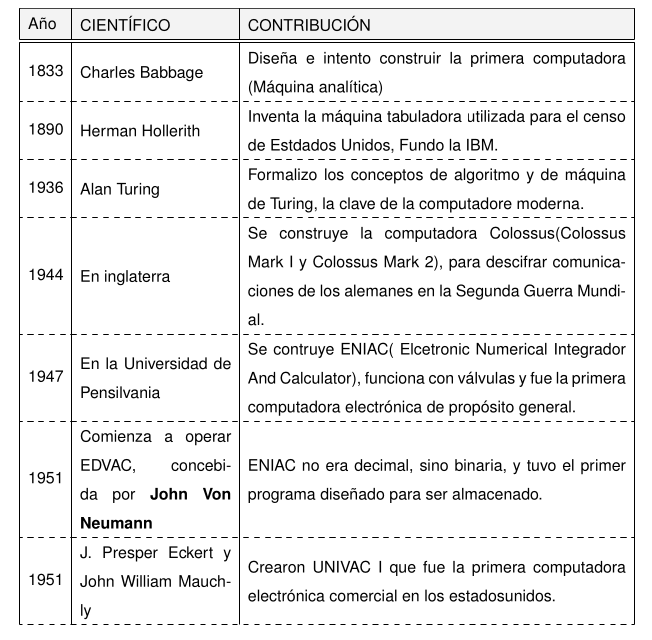
\includegraphics[width=180px]{./images/historia1.png}
\caption{Historia del comptuador}
\end{figure}
\end{frame}


\begin{frame}[label={sec:org211954d}]{\textit{<2021-09-15 Wed 09:00>--<2021-09-15 Wed 10:00> } Historia del computador}
\begin{figure}[htbp]
\centering
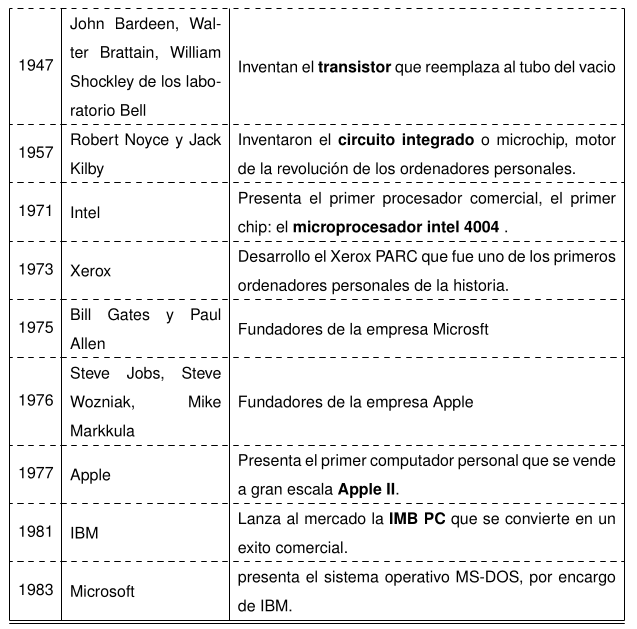
\includegraphics[width=180px]{./images/historia2.png}
\caption{Historia del comptuador}
\end{figure}
\end{frame}


\begin{frame}[label={sec:org58c1052}]{\textit{<2021-09-15 Wed 09:00>--<2021-09-15 Wed 10:00> } Arquitectura del computador}
\begin{block}{Diagrama de la arquitectura Von Neuman}
\begin{figure}[htbp]
\centering
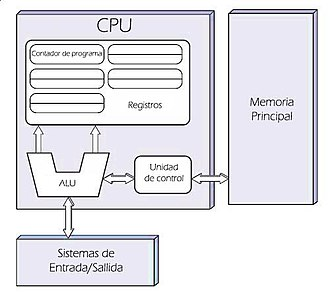
\includegraphics[width=180px]{./images/Arquitecturaneumann.jpg}
\caption{Arquitectura Von Neumann}
\end{figure}
\end{block}
\end{frame}


\begin{frame}[label={sec:orgadf21e8}]{El software.}
\begin{itemize}
\item ¿Que es el software?
\item ¿Qué es numeración binaria?
\item ¿Que es sitemas de númeración?
\item ¿Como transformas de un sistemas de numeración a otro?
\item Ejercicio para el fin de semana.
\end{itemize}
\end{frame}


\begin{frame}[label={sec:org1f1fcb6}]{Sistema de Numeración Binaria}
\begin{figure}[htbp]
\centering
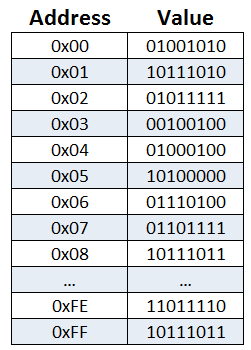
\includegraphics[width=120px]{./images/memoria.png}
\caption{La memoria del computador}
\end{figure}
\end{frame}

\begin{frame}[label={sec:orgd7a0206}]{Sistemas de Numeración}
\begin{itemize}
\item Sistema de númeración Binaria.
\item Sistema de númeración Octal.
\item Sistema de númeración Decimal.
\item Sistema de númeración Exadecimal.
\end{itemize}
\end{frame}

\begin{frame}[label={sec:org0339e3d}]{Conversión Sistemas de Númeración.}
\begin{figure}[htbp]
\centering
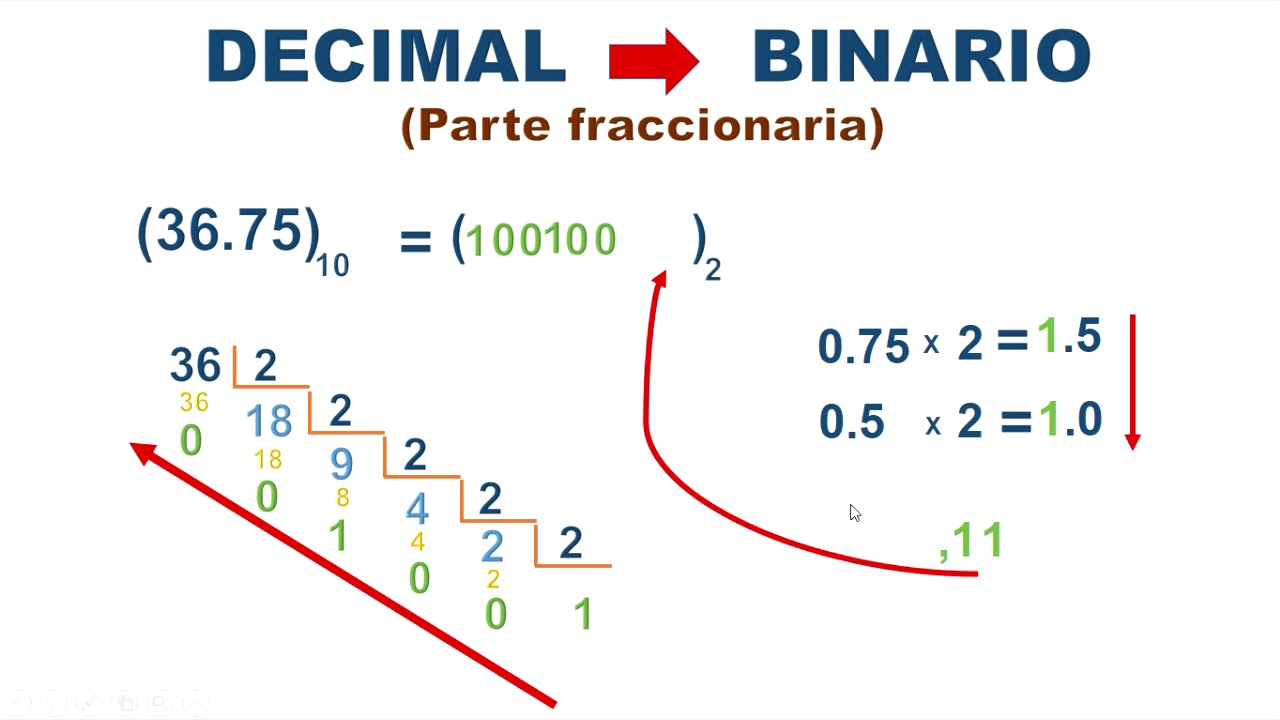
\includegraphics[width=250px]{./images/DecimalBinario.jpg}
\caption{Conversión Sistemas de Númeración.}
\end{figure}
\end{frame}



\begin{frame}[label={sec:org69dc9b7}]{Lenguaje de programación}
\begin{figure}[htbp]
\centering

\includegraphics[width=.9\linewidth]{./images/LenguajesDeProgramacion.jpg}
\caption{Todos los lenguajes de programación}
\end{figure}
\end{frame}
\begin{frame}[label={sec:orge773110}]{Lenguaje a utilizar para esta curso.}
\begin{figure}[htbp]
\centering
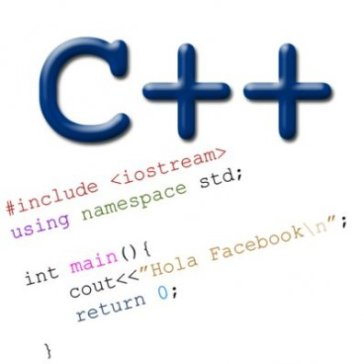
\includegraphics[width=150px]{./images/cpp.jpg}
\caption{Lenguaje a utilizar en este}
\end{figure}
\end{frame}

\section{UNIDAD 2: Nociones de linux, vim, clang}
\label{sec:orgac29f85}
\begin{frame}[label={sec:orgcf420ec}]{Introducción a Linux y termux}
\end{frame}
\begin{frame}[label={sec:orgf1c43b8}]{Paquetes de Linux: ejercicios prácticos}
\end{frame}
\begin{frame}[label={sec:org9b8c9e3}]{Introducción a Vim  y sus comandos.}
\end{frame}
\begin{frame}[label={sec:org75f8fad}]{Ejercicios prácticos con Vim.}
\end{frame}
\section{UNIDAD 3: Metodología de la programación y Diagrama de flujo}
\label{sec:orge7432b9}
\begin{frame}[label={sec:orgc6f9911}]{Introducción a al programación}
\end{frame}
\begin{frame}[label={sec:orga12c989}]{Ciclo de Vida del Software.}
\end{frame}
\begin{frame}[label={sec:org294e302}]{Diagrama de Flujo: Hola Mundo.}
\end{frame}
\section{Semana de Evuación sumativa}
\label{sec:org8705eb1}
\section{UNIDAD 4: Programación en C++: Introducción.}
\label{sec:org7183623}
\begin{frame}[label={sec:orgfa188f0}]{Elementos básicos en un programa en c++.}
\begin{block}{Básicos.}
\begin{itemize}
\item Palabras reservadas (main, return, if while, do ,.. etc.).
\item Identificadores (nombre de variables, nombre de funciones, nombres de programas, etc.).
\item Caracteres especiales (coma,punto,punto y coma, etc.).
\item Constantes.
\item Variables.
\item Expresiones.
\item Instrucciones.
\end{itemize}
\end{block}
\begin{block}{Derivados.}
\begin{itemize}
\item Bucles.
\item Contadores.
\item Acumuladores.
\item Interruptores.
\item Estructuras (secuenciales, selectivas, repetitivas).
\end{itemize}
\end{block}
\end{frame}
\begin{frame}[label={sec:org71eb7cf}]{Un programa básico en C++.}
\begin{itemize}
\item 
\end{itemize}
\end{frame}
\section{UNIDAD 5: Flujo de control :Selección y Repetición.}
\label{sec:org207062c}
\begin{frame}[label={sec:org0670b4c}]{Estructuras de control son:}
\begin{block}{Estructura de selección}
\begin{itemize}
\item Estructura if-else
\item Estructura if
\item Estructura switch
\end{itemize}
\end{block}
\begin{block}{Estructura de repetición}
\begin{itemize}
\item Estructura do-while
\item Estructura while
\item Estructura for
\end{itemize}
\end{block}
\end{frame}
\begin{frame}[label={sec:org519cd54}]{Estructura de selección (if-else).}
\begin{columns}
\begin{column}{0.4\columnwidth}
\begin{center}
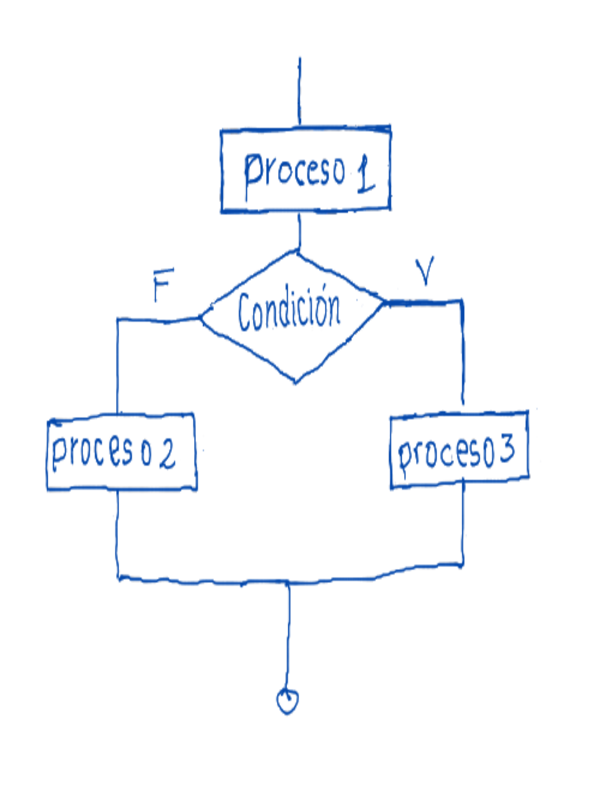
\includegraphics[width=.9\linewidth]{./images/codigo/ifsino.png}
\end{center}
\end{column}
\begin{column}{0.6\columnwidth}
\begin{center}
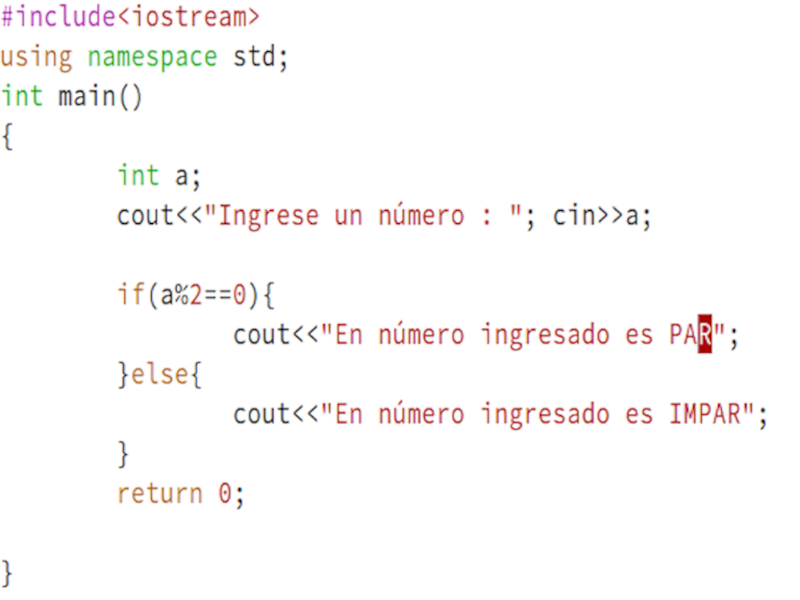
\includegraphics[width=.9\linewidth]{./images/codigo/code-ifsino.png}
\end{center}
\end{column}
\end{columns}
\end{frame}

\begin{frame}[label={sec:org0e1347c}]{Estructura de control (if-else)}
\begin{columns}
\begin{column}{0.4\columnwidth}
\begin{center}
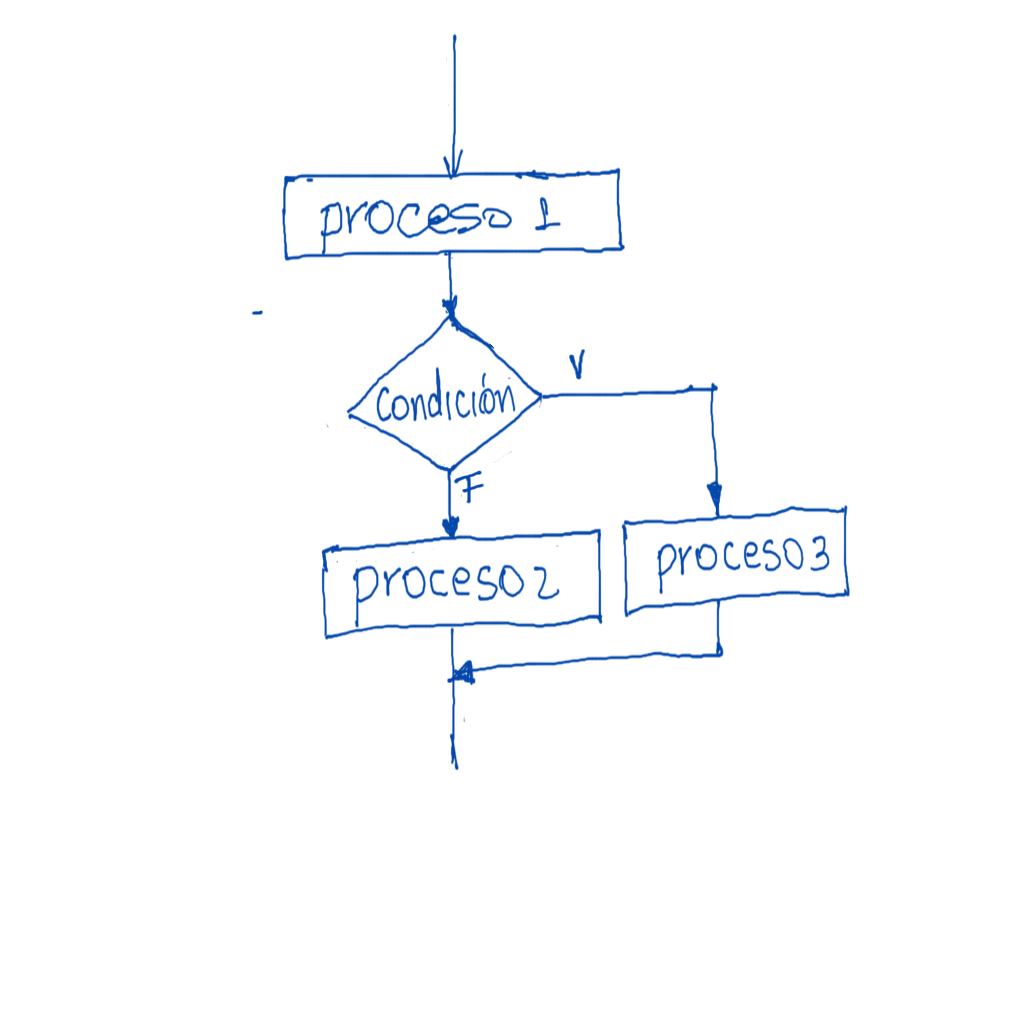
\includegraphics[width=.9\linewidth]{./images/codigo/ifsino2.png}
\end{center}
\end{column}

\begin{column}{0.6\columnwidth}
\begin{center}
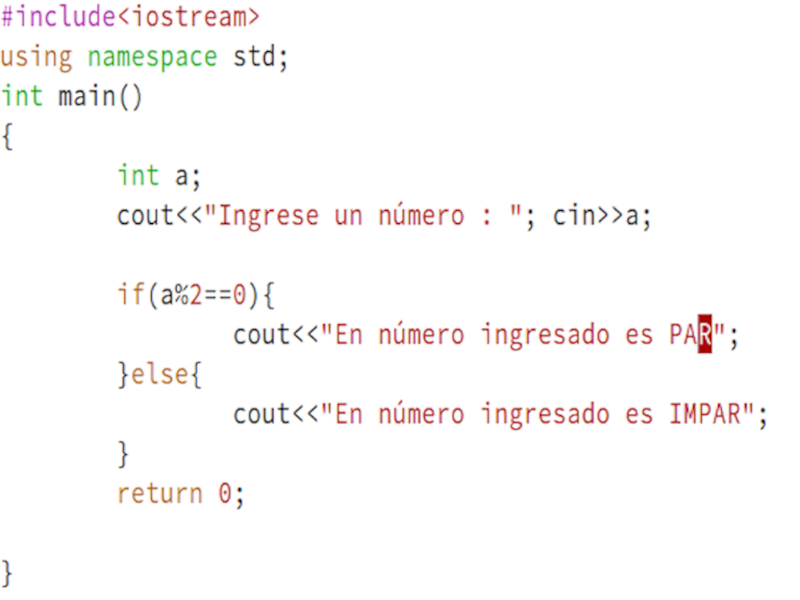
\includegraphics[width=.9\linewidth]{./images/codigo/code-ifsino.png}
\end{center}
\end{column}
\end{columns}
\end{frame}


\begin{frame}[label={sec:orgfb8e82e}]{Estructura de control (if)}
\begin{columns}
\begin{column}{0.4\columnwidth}
\begin{center}
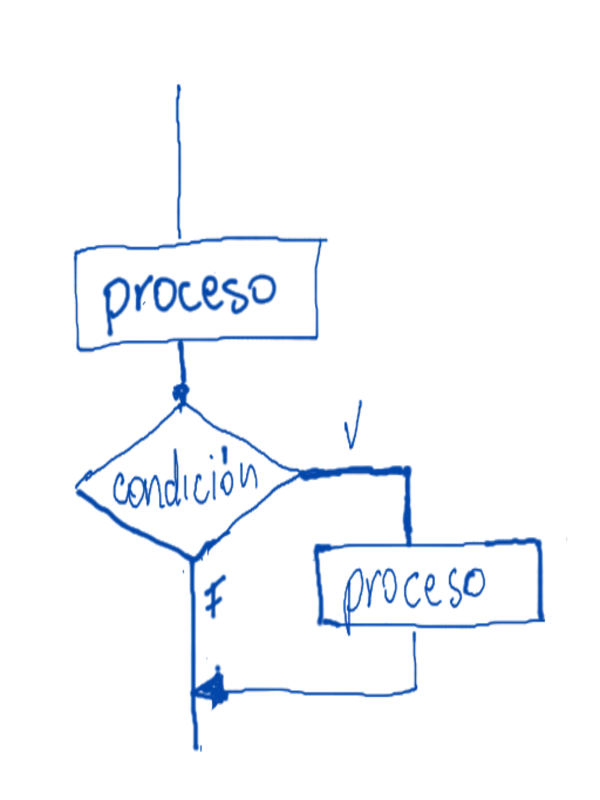
\includegraphics[width=.9\linewidth]{./images/codigo/if.png}
\end{center}
\end{column}
\begin{column}{0.6\columnwidth}
\begin{center}
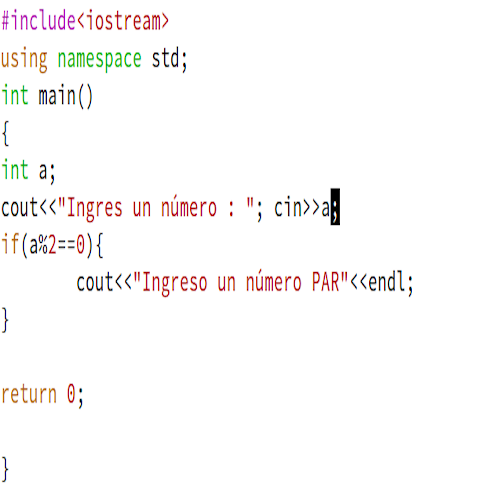
\includegraphics[width=.9\linewidth]{./images/codigo/code-if.png}
\end{center}
\end{column}
\end{columns}
\end{frame}


\begin{frame}[label={sec:org5afb780}]{Estructura de control (if excluyentes)}
\begin{columns}
\begin{column}{0.4\columnwidth}
\begin{center}
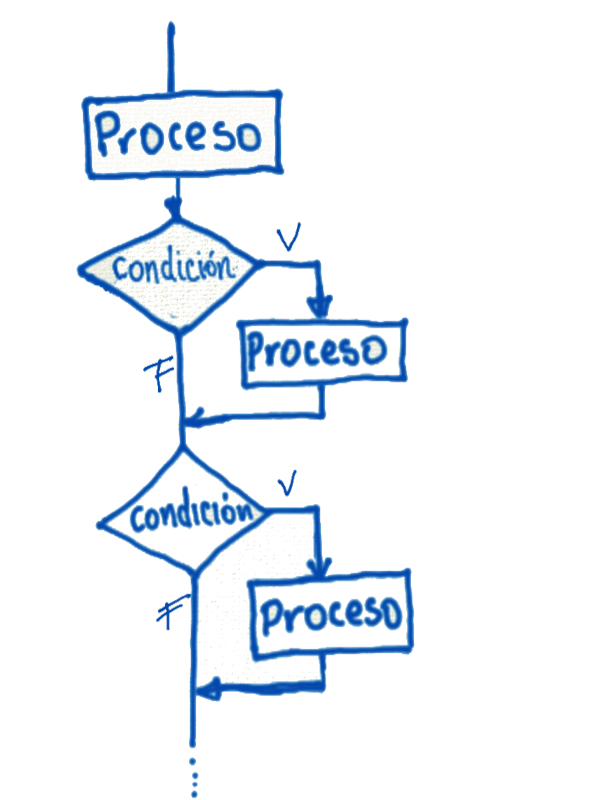
\includegraphics[width=.9\linewidth]{./images/codigo/ifexcluyentes.png}
\end{center}
\end{column}

\begin{column}{0.6\columnwidth}
\begin{center}
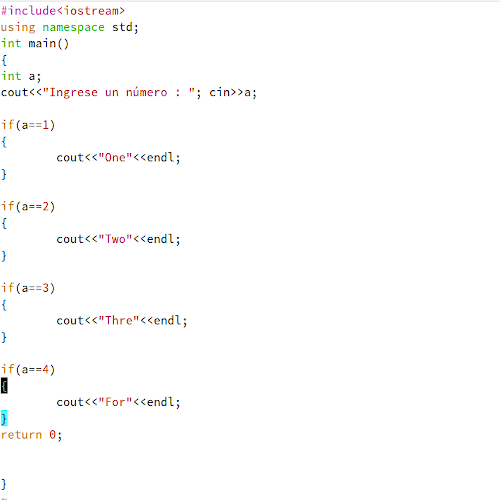
\includegraphics[width=.9\linewidth]{./images/codigo/code-ifexcluyentes.png}
\end{center}
\end{column}
\end{columns}
\end{frame}



\begin{frame}[label={sec:org154be20}]{Estructura de control (switch)}
\begin{columns}
\begin{column}{0.4\columnwidth}
\begin{center}
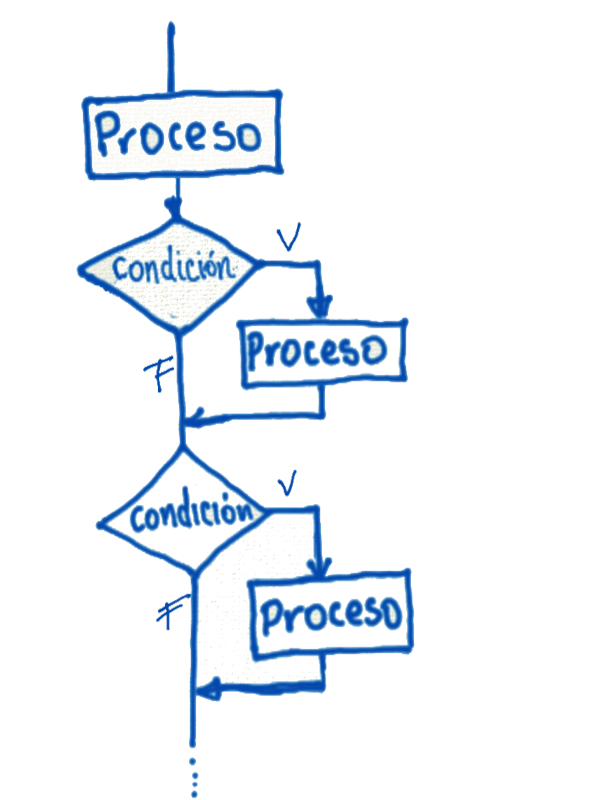
\includegraphics[width=.9\linewidth]{./images/codigo/ifexcluyentes.png}
\end{center}
\end{column}

\begin{column}{0.6\columnwidth}
\begin{center}
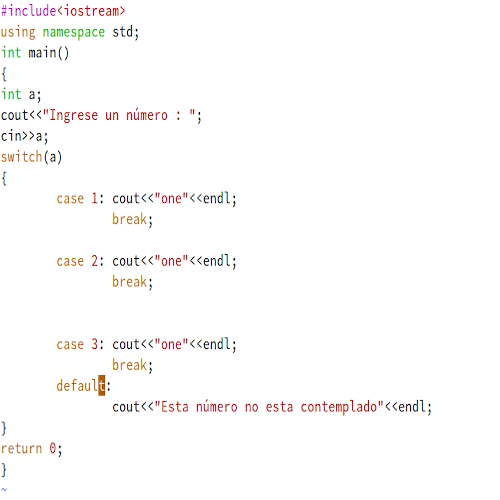
\includegraphics[width=.9\linewidth]{./images/codigo/code-switch.png}
\end{center}
\end{column}
\end{columns}
\end{frame}





\begin{frame}[label={sec:org5daadb0}]{Estructura de control (do-while)}
\begin{columns}
\begin{column}{0.4\columnwidth}
\begin{center}
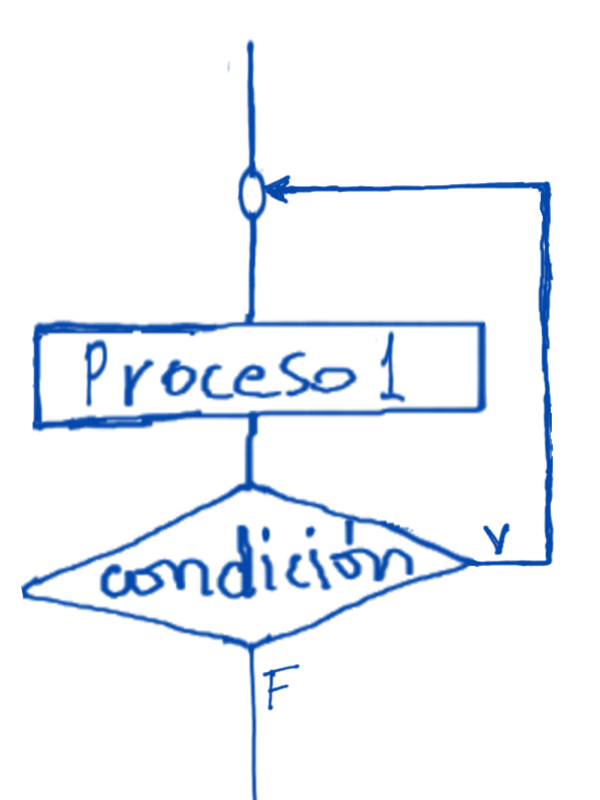
\includegraphics[width=.9\linewidth]{./images/codigo/dowhile.png}
\end{center}
\end{column}
\begin{column}{0.6\columnwidth}
\begin{center}
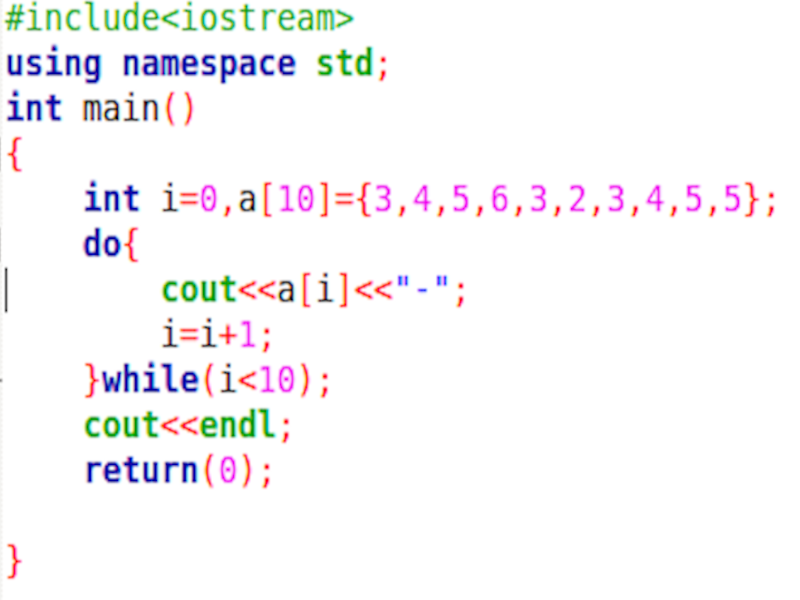
\includegraphics[width=.9\linewidth]{./images/codigo/code-dowhile.png}
\end{center}
\end{column}
\end{columns}
\end{frame}


\begin{frame}[label={sec:orgfe21858}]{Estructura de control (while)}
\begin{columns}
\begin{column}{0.4\columnwidth}
\begin{center}
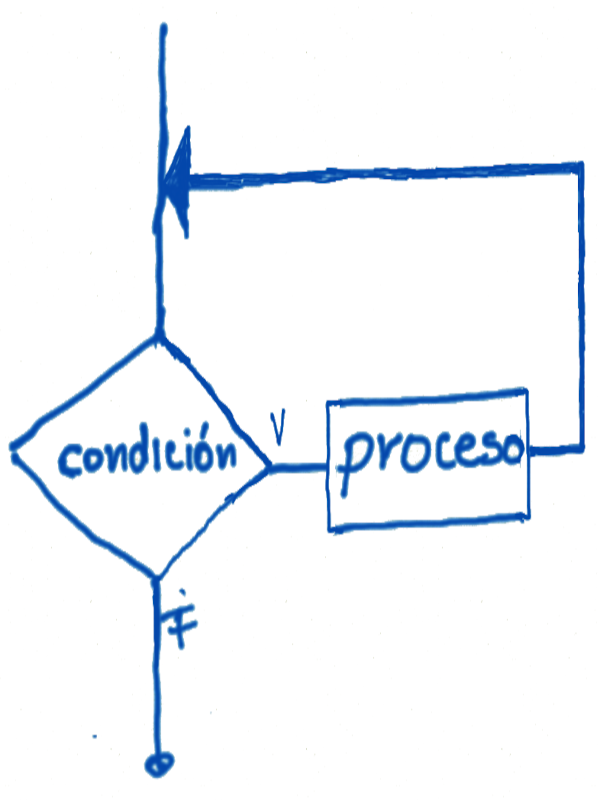
\includegraphics[width=.9\linewidth]{./images/codigo/for.png}
\end{center}
\end{column}

\begin{column}{0.6\columnwidth}
\begin{center}
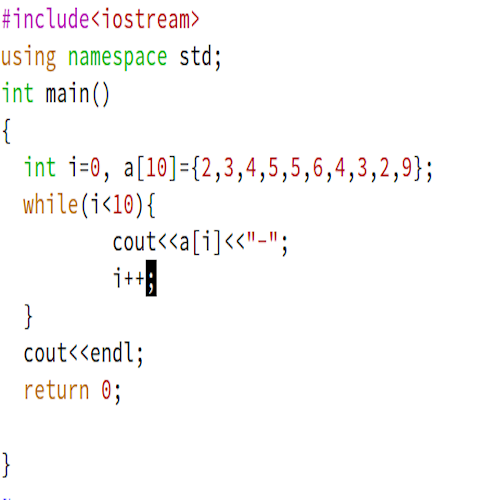
\includegraphics[width=.9\linewidth]{./images/codigo/code-while.png}
\end{center}
\end{column}
\end{columns}
\end{frame}


\begin{frame}[label={sec:org56fc702}]{Estructura de control (for)}
\begin{columns}
\begin{column}{0.4\columnwidth}
\begin{center}
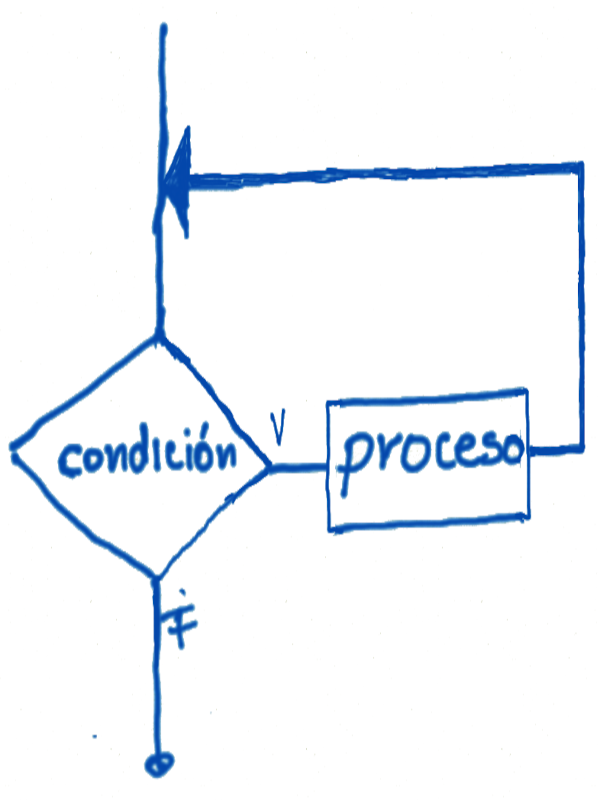
\includegraphics[width=.9\linewidth]{./images/codigo/for.png}
\end{center}
\end{column}
\begin{column}{0.6\columnwidth}
\begin{center}
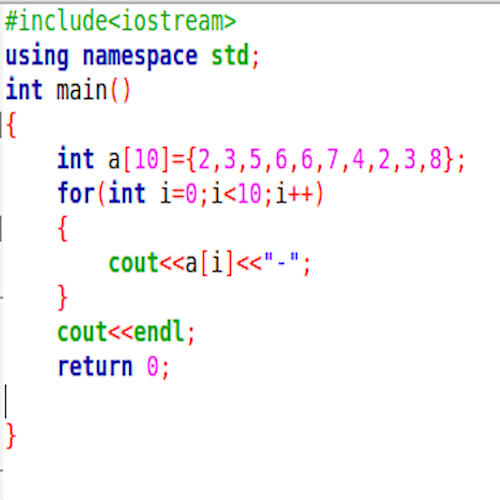
\includegraphics[width=.9\linewidth]{./images/codigo/code-for.png}
\end{center}
\end{column}
\end{columns}
\end{frame}


\section{UNIDAD 6: Flujo de control II: Estructura Repetiviva}
\label{sec:org161beef}
\begin{frame}[label={sec:orgb4bf71b}]{org-mode + beamer =  love}
\begin{columns}
\begin{column}{0.7\columnwidth}
<example block>
\end{column}
\begin{column}{0.3\columnwidth}
\begin{block}{Simple block}
it's that easy!
\end{block}
\end{column}
\end{columns}
\end{frame}



\section{UNIDAD 7: Funciones y librerias personales}
\label{sec:orgd700567}
\begin{frame}[label={sec:orgf2d9ac3}]{monolítico}
\begin{figure}[htbp]
\centering
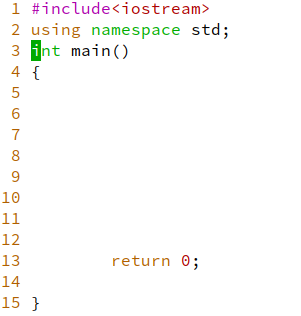
\includegraphics[width=0.5\linewidth]{./images/codigo/monolitico-1.png}
monolítico-1.cpp
\end{figure}
\end{frame}
\begin{frame}[label={sec:org61122a7}]{monolítico2}
\begin{figure}[htbp]
\centering
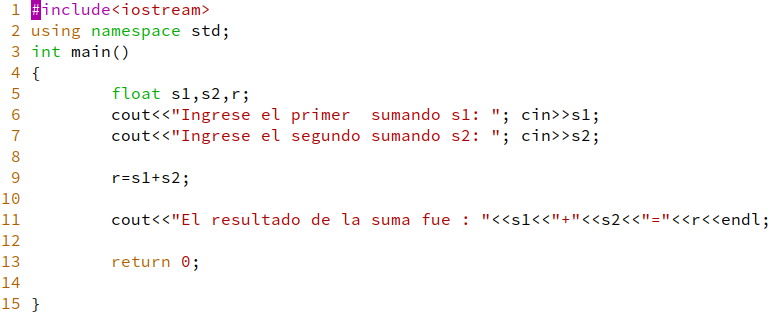
\includegraphics[width=1.1\linewidth]{./images/codigo/monolitico-2.png}
monolítico-2.cpp
\end{figure}
\end{frame}
\begin{frame}[label={sec:orge1e38bd}]{Programación monolítica con funciones}
\begin{figure}[htbp]
\centering
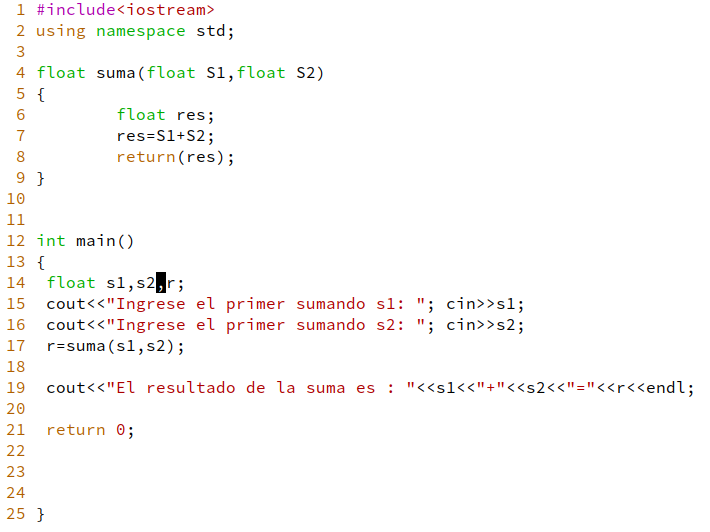
\includegraphics[width=.9\linewidth]{./images/codigo/funcion1.png}
funcion-1.cpp
\end{figure}
\end{frame}
\begin{frame}[label={sec:org78d3642}]{Programación monolítica con prototipo de funciones}
\begin{figure}[htbp]
\centering
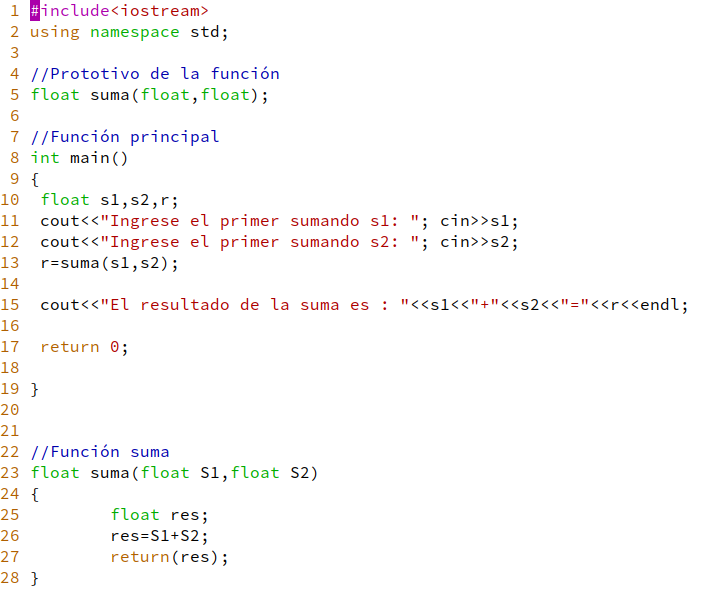
\includegraphics[width=0.8\linewidth]{./images/codigo/funcion2.png}
funcion-2.cpp
\end{figure}
\end{frame}

\begin{frame}[label={sec:org3d0ef5d}]{Programa monolítico.}
\begin{columns}
\begin{column}{0.45\columnwidth}
\begin{figure}[htbp]
\centering
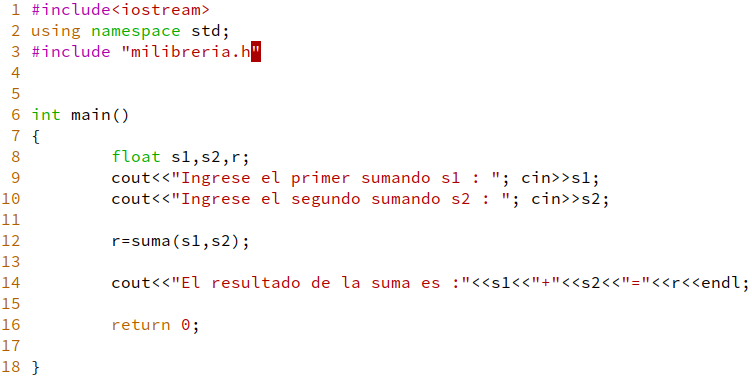
\includegraphics[width=1.3\textwidth]{./images/codigo/principal.png}
principal.cpp
\end{figure}
\end{column}
\begin{column}{0.45\columnwidth}
\begin{figure}[htbp]
\centering
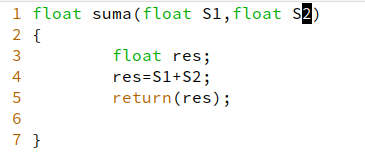
\includegraphics[width=0.7\linewidth]{./images/codigo/milibreria.png}
milibreria.h
\end{figure}
\end{column}
\end{columns}
\end{frame}



\section{UNIDAD 8: Programación Orientada a Objetos: clases}
\label{sec:orgc84f40b}
\end{document}